\documentclass[12pt,fleqn]{article}\usepackage{../../common}
\begin{document}
Ders 15

Dersimizin kaos bolumune geldik. Kaosu bir su carki orneginde gorecegiz, su
carkini biliyoruz, eger bir yerde dogal su akisi varsa oraya cark konur, su
duserken carki dondurur.

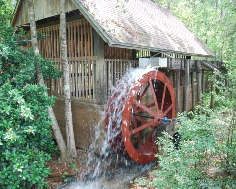
\includegraphics[width=10em]{waterwheel.jpg}

Isleyecegimiz su carki biraz degisik yanliz, 

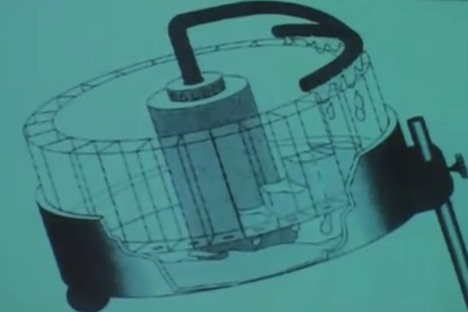
\includegraphics[width=20em]{15_01.jpg}

Bu tam bir su carkina benzemiyor biliyorum. Bu carkta cark kismi yatay,
mekanizmanin altinda. Fakat bu yatay kisim kaldirilip indirilebiliyor, yani
yuzeye bir egim halinde tutulabiliyor, bu egimi yandaki boru uzerindeki bir
vida ile ayarlayabiliyoruz. Sistemimizin bir parametresi bu olacak. 













Kaynaklar

Strogatz, Video, \url{https://www.youtube.com/watch?v=7iNCfNBEJHo}

\end{document}











